%%% -*-LaTeX-*-

\chapter{Theoretical Background on Morse Theory}
\label{ch:theory}

Although we have introduced numerous topological constructs in previous chapters, we now provide a more formal treatment of them in this chapter and discuss implementation issues regarding how to approximate on unstructured datasets existing in the high-dimensional setting.

Because we are interested in functional relationships, we limit ourselves to Morse theory.
%
Morse theory~\cite{Matsumoto2002,Milnor1973,Morse1949} is a subtopic of differentiable topology that analyzes the topology of manifolds under differentiable functions.
%
Specifically, a class of functions, so-called Morse functions, are used to study such concepts as the critical points, levelsets and gradient behavior of manifold spaces.
%
Therefore, the remainder of this section will address each one of these categories in turn.

\begin{defn}
  \textbf{Morse function} - A smooth function with no degenerate critical points, and every critical point is isolated.
\end{defn}

\section{Critical Points}

\begin{lem} Morse Lemma - Let $\mathbf{p}$ be a nondegenerate critical point of $f : A \rightarrow \mathbb{R}$ where $A$ is an $n$-manifold, then there exists a local coordinate system $(x_1,...,x_n$) in a neighborhood of $\mathbf{p}$ such that $x_i(\mathbf{p}) = 0$ and is represented in a \textbf{standard form}:

\begin{equation}
f = f(\mathbf{p}) - \sum_{i=1}^{\lambda}x_i^2 + \sum_{j=\lambda+1}^n x_j^2, \{\lambda \in \mathbb{Z} | 0 \leq \lambda < n\}
\end{equation}
\end{lem}

The symbol $\mathbb{Z}$ is taken to mean the set of all integers.
%
This lemma claims that we can fit a parabolic function locally around each nondegenerate critical point with respect to each dimension to represent $f$ where a given number of dimensions will have downward-facing parabolas and the remaining will have upward-facing parabolas.
%
The parameter $\lambda$ specifies how many of each occur for the given critical point, and Figure~\ref{fig:critical_points} shows the three cases for critical points of a two-dimensional function.

\begin{defn}
\textbf{Critical point index} - Given the standard form above for a critical point $\mathbf{p}$, the value of $\lambda$ represents the index of $\mathbf{p}$ for $f$.
\end{defn}

A zero-index critical point represents a local minimum, since locally the function is increasing in every direction about the point. Critical points of index $k$ where $0 < k < d$ and $d$ is the dimension of the manifold are known as $k$-saddles.
%
Saddles are so named for the shape they resemble in the two-manifold case, and in that case exhibit alternating sign of the directional derivative when traversing a clockwise/counterclockwise path around the saddle.
%
The $d$-index critical points represent local maxima where locally the function is decreasing in every direction. Locally, consider a parabola that opens downward when considering each dimension in isolation.

\begin{figure}[b]
  \centering
  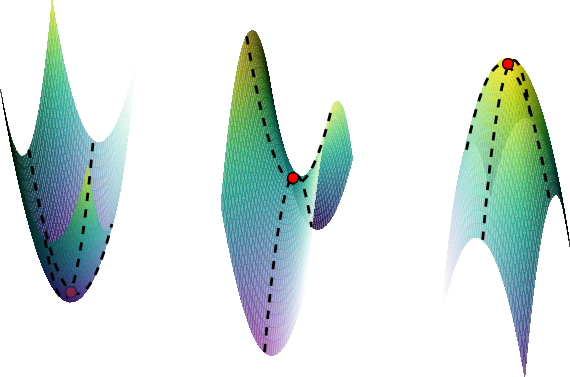
\includegraphics[width=0.5\textwidth]{figs/chap4/criticalPoints}
  \caption[Critical Points of Varying Index]{The standard form of critical points is summarized in the two-dimensional case by visualizing parabolic curves along each dimensional axis. Here we see from left, a zero-index minimum with zero downward facing parabolas, a one-saddle with one downward facing parabola, and a two-index maximum with two downward facing parabolas.}
  \label{fig:critical_points}
\end{figure}

\section{Morse and Morse-Smale Complexes}

As stated previously, we can also use Morse theory to partition a space according to uniform gradient flow.
%
For a given location in the domain space, one can follow the gradient direction to a local maximum.
%
Likewise, following the negative gradient direction leads to a local minimum.
%
The path defined by following the gradient in both directions is known as an integral line.

\begin{defn}
  \textbf{Integral line} - A curve, $l(t)$ such that $\frac{d}{dt}l(t) = \nabla f(l(t)), \forall t \in \mathbb{R}$. In words, $l$ is a path whose tangent is parallel to the gradient of $f$ everywhere it is defined.
\end{defn}

\begin{defn}
  \textbf{Origin} - $\lim\limits_{t\to-\infty} l(t)$
\end{defn}

\begin{defn}
  \textbf{Destination} - $\lim\limits_{t \to \infty} l(t)$
\end{defn}

Integral lines on Morse functions have several useful properties:

\begin{itemize}
\item Integral lines are disjoint or the same.
\item Integral lines cover all of $\mathbb{M}$.
\item The origin and destination of an integral line are critical points of $f$.
\item Integral lines are monotonic and thus $org(l) \neq dest(l)$.
\item Each point in $\mathbb{M}$ has one and only one integral line passing through it.
\end{itemize}

Using the origin or destination as classifiers, we can partition the data into either ascending or descending manifolds, which are defined below.

\begin{defn}
  \textbf{Ascending/unstable Manifold} - The set of points in a manifold whose integral lines have the same origin.
\end{defn}

\begin{defn}
  \textbf{Descending/stable Manifold} - The set of points in a manifold whose integral lines have the same destination.
\end{defn}

% \subsection{Morse Complex}

\begin{defn}
 \textbf{Morse Complex} - A partition of a manifold into equivalence classes based on the destination of integral lines: $\{x,y \in A | x~y \Rightarrow dest(x) = dest(y)\}$. Also, the complex of descending manifolds of $f$.
\end{defn}

By inverting the function, $-f$, and computing the Morse complex, we can obtain the complex of ascending manifolds of the original function $f$.
%
By combining both complexes, we can obtain the Morse-Smale complex that partitions the space into areas of distinct origin and destination pairs.

% \subsection{Morse-Smale Complex}

\begin{defn}
\textbf{transverse intersection} - Consider two submanifolds of $\mathbb{C}$, $\mathbb{A}$ and $\mathbb{B}$. $\{\forall \mathbf{x} \in \mathbb{A} \cap \mathbb{B}: T_{\mathbb{A}} + T_{\mathbb{B}} = T_{\mathbb{C}} \text{ or } \mathbb{A} \cap \mathbb{B} = \emptyset\}$ where $T_{X}$ represents the tangent space of $X$.
%
Thus, if $\mathbb{A}$ and $\mathbb{B}$ intersect, they do so such that their combined tangent maps spans the tangent space of the ambient manifold $\mathbb{C}$.
\end{defn}

\begin{defn}
\textbf{Morse-Smale function} - A Morse function whose ascending and descending manifolds intersect transversally.
\end{defn}

\begin{defn}
\textbf{Morse-Smale Complex} - The complex formed by the intersection of the Morse complexes of $f$ and $-f$.
\end{defn}

In this way, a Morse-Smale complex identifies each location in the manifold with a local minimum (origin) and a local maximum (destination).
%
Boundaries between cells in a $d$-manifold are themselves $(d-1)$-manifolds that connect local minima to one-saddles, one-saddles to two-saddles, etc., and $(d-1)$-saddles to local maxima.

% \subsection{Piecewise Linear}

This theory works well when applied to smooth fields, but some gaps must be addressed in order to perform such a decomposition on arbitrary dimensional point cloud data.
%
Namely, in order to identify each point to an ascending or descending manifold, we must trace the integral lines through the available data, which implies that we have some connectivity structure among the data points.
%
In order to do this, we employ concepts from either the piecewise linear case~\cite{EdelsbrunnerLetscherZomorodian2002} or discrete Morse theory~\cite{Forman2002}.
%
Gyulassy has addressed many of these issues when working with structured and unstructured grids in low-dimensional spaces~\cite{Gyulassy2008}, and more recently Gerber et al.~\cite{GerberBremerPascucci2010} have developed an algorithm for approximating gradient on arbitrary dimensional point clouds.
%
In this work, we utilize the latter algorithm and so explain it in further detail with proposed improvements.

\clearpage
\section{Arbitrary Dimensional Approximation of the Morse-Smale Complex}
\label{sec:approximationMSC}

We treat the problem of computing the Morse-Smale complex as computing two Morse complexes, one to compute descending manifolds (Morse complex of $f$) and another to compute ascending manifolds (Morse complex of $-f$).
%
As mentioned, we must impose a connectivity structure on the data in order to estimate the gradient.
%
For this, a neighborhood graph is used that represents a one-skeleton of the manifold.
%
The original works of Gerber et al.~\cite{GerberBremerPascucci2010,GerberPotter2012,GerberRubelBremer2011} used a $k$-nearest neighbor graph, but more recently, Correa and Lindstrom~\cite{CorreaLindstrom2011} explored the use of empty region graphs that have been shown to provide better results in extracting topological features from sparsely sampled datasets.
%
Under specific sampling densities, the $k$-nearest neighbor can tend to bias certain directions where the point density is higher.
%
The empty region graphs, on the other hand, validate edges by ensuring no points lie in a region encompassing the edge.
%
The shape of this region varies according to the specific type of graph used, but the end result is a less biased and more uniform distribution of edges over the hypersphere of directions emanating from any given point.
%
Cone graphs, introduced in Section~\ref{sec:bg_cones}, represent a third family of graphs that could potentially be used for imposing a structure similar to that achieved by the empty region graphs.
%
We explore a direct comparison of these three graph types for extracting topology in Chapter~\ref{ch:graphs}.
%
In all experiments where this method is employed in this dissertation, we denote the type of graph used.

The algorithm is quite straightforward once the graph is imposed on the data.
%
We visit each point and estimate its positive and negative gradient directions according to the function value difference between itself and each of its neighbors divided by the distance between the two points.
%
The largest magnitude positive and negative values belong to the edges that represent the discretized integral line.
%
If a point has no values of lesser value, it is a local minimum.
%
Equally, if a point has no values of higher value, it is labeled a local maxima.
%
We can then trace the positive integral line from each data point up to a local maximum, and trace the negative integral line down to a local minimum.
%
We retain the indices of the identified local minimum and maximum, and this pair of indices represents the Morse-Smale cell to which this point belongs.
%
Note that we can utilize a union-find data structure to prevent repeating traversals.
%
This short-cutting amortizes the cost of finding extrema to be a near linear complexity operation.

As was pointed out in the end of Chapter~\ref{ch:definitions}, gradient inconsistencies such as crossing integral lines can form if the graph has crossing edges.
%
This type of error can be avoided by detecting and pruning such edges from the graph or by using a graph that strictly prevents them.
%
In most cases, the inconsistencies this causes are minor, and the time needed to detect and remove such edges can often outweigh the potential existence of these inconsistencies.
%
Furthermore, as dimensionality increases, the likelihood of edges crossing reduces as the space becomes sparser, and any set of four points have to meet an additional coplanar requirement for each dimension added.
%
% In pratical settings, we begin with an approximate $k$-nearest neighbor graph where $k$ is intentionally set higher than expected and prune it with one of the empty region criteria from Correa and Lindstrom's work to achieve computational efficiency.

Figure~\ref{fig:mscAlgorithm} shows the three-step process of the discretized Morse-Smale complex algorithm, including application of a graph structure, tracing gradients to local extrema, and the third step discussed in the next section, persistence simplification, which essentially denoises the results.

\begin{figure}[b]
  \centering
  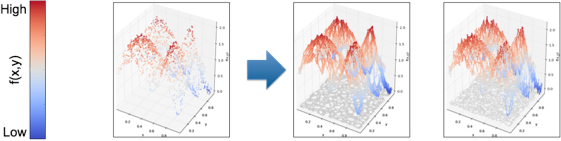
\includegraphics[width=0.75\textwidth]{figs/chap4/amscStep1}
  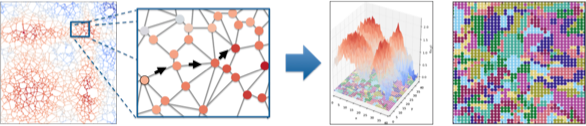
\includegraphics[width=0.75\textwidth]{figs/chap4/amscStep2}
  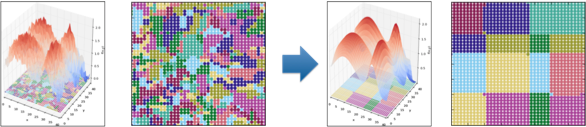
\includegraphics[width=0.75\textwidth]{figs/chap4/amscStep3}
  \caption[Illustration of the Morse-Smale approximation for unstructured data]{The three main steps in the approximation algorithm for computing the Morse-Smale complex. They are, from top to bottom: construction of graph on input data, gradient tracing to local extrema, and construction of hierarchy of features allowing for simplification of the extracted topology.}
  \label{fig:mscAlgorithm}
\end{figure}

\subsection{Persistence Simplification}
At this point, we are able to identify topological features as critical points in the function space.
%
When considering even low-dimensional examples such as a two-dimensional terrain, it is clear that not all of the topological features are of equal significance.
%
Thus, we seek some way by which we can sort the topological features in both the Reeb graph and  Morse-Smale complex setting in some way so as to capture this ``significance.''
%
Doing so affords us the opportunity to deconstruct the topology into a hierarchical representation whereby we can look at the topology at different scales of resolution, allowing us to denoise the results.

The notion of significance that we use is taken from the field of persistent homology.
%
Persistent homology can be applied to nonfunctional point cloud data as in the simplicial complex case considered by Carlsson and Ghrist~\cite{Carlsson2009,Ghrist2009}.
%
In such a case, a filtration of a simplicial complex is analyzed in order to track the birth and death of connected components.
%
We are concerned with the persistence of features occurring in scalar function data as presented in the survey of Edelsbrunner and Harer~\cite{EdelsbrunnerHarer2008}.

In order to describe persistence, we begin with the simple 1D case.
%
Let $f: \mathbb{R} \rightarrow \mathbb{R}$ be a smooth function with nondegenerate critical points, meaning each critical point is either a local minimum or a local maximum (i.e., there are no inflection points).
%
The sublevel sets of $f$ change connectivity only when we pass critical values.
%
That is, when we pass a local minimum value, a new connected component is created or ``born,'' and when we pass a local maximum value, two connected components merge together.
%
In this way, we can pair critical points.
%
When a new component is born, the local minimum that created it is its representative.
%
Upon passing a local maximum and merging two components, the maximum is paired with the higher valued local minimum representing the formerly separate connected components.
%
The pair is assigned a persistence value equal to the function value difference of the local maximum and local minimum.
%
The merged connected component retains the lower valued local minimum as its representative.
%
Once a local minimum is paired, it will not be paired again because there is no longer a connected component represented by it.
%
A two-dimensional example is given in Figure~\ref{fig:persistenceFill}.

\begin{figure}[t]
  \centering
  \raisebox{-.5\height}{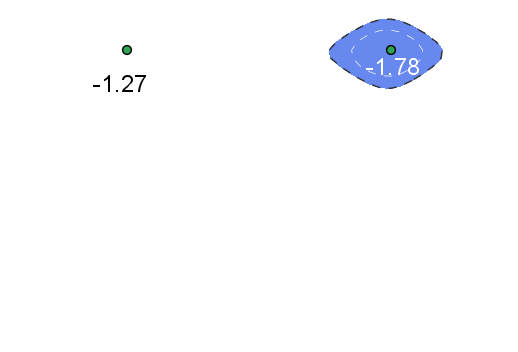
\includegraphics[width=0.2\textwidth]{figs/chap4/persistence1}}
  \raisebox{-.5\height}{
\includegraphics[width=0.04\textwidth]{figs/chap4/arrow}}
  \raisebox{-.5\height}{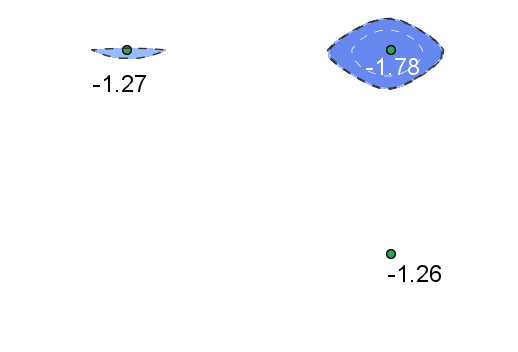
\includegraphics[width=0.2\textwidth]{figs/chap4/persistence2}}
  \raisebox{-.5\height}{
\includegraphics[width=0.04\textwidth]{figs/chap4/arrow}}
  \raisebox{-.5\height}{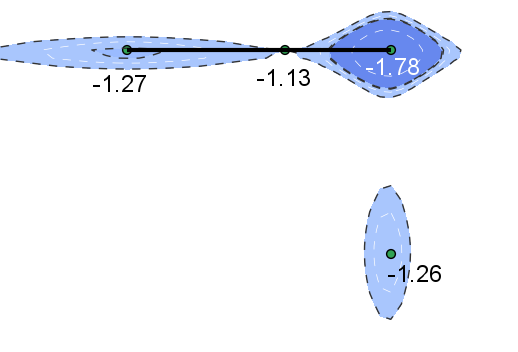
\includegraphics[width=0.2\textwidth]{figs/chap4/persistence3}}
  \raisebox{-.5\height}{
\includegraphics[width=0.04\textwidth]{figs/chap4/arrow}}
  \raisebox{-.5\height}{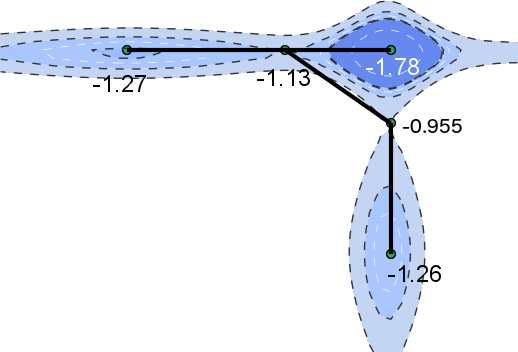
\includegraphics[width=0.2\textwidth]{figs/chap4/persistence4}}
  \caption[Illustration of Persistence Pairing]{One way of understanding
  persistence simplification is to consider the flooding of a terrain.
  %
  As we progress from left to right, we see additional components being born and then the merging of separate components into single components.
  %
  These merge events occur at the levelsets of the saddle points, and the attached local minima become a persistence pairing with the persistence value being the difference between the saddle's function value and the maximum function value of the two minima associated.
  %
  In the case of the third image, this value would be $-1.13-(-1.27)=0.14$ whereas the merge in the fourth image yields a persistence value of $-0.955-(-1.26)=0.305$.}
  \label{fig:persistenceFill}
\end{figure}

A common tool for visualizing these persistence pairings is the persistence diagram (see Figure~\ref{fig:persistenceDiagram}), which maps the function value of the local minimum (the `birth' point) on the horizontal axis and the function value of the local maximum (the `death' point) on the vertical axis.
%
No point will lie below the identity $y=x$ as a pair must be born before it dies.
%
The persistence of a pair is given by the vertical distance to the identity line.

\begin{figure}[t]
  \centering
  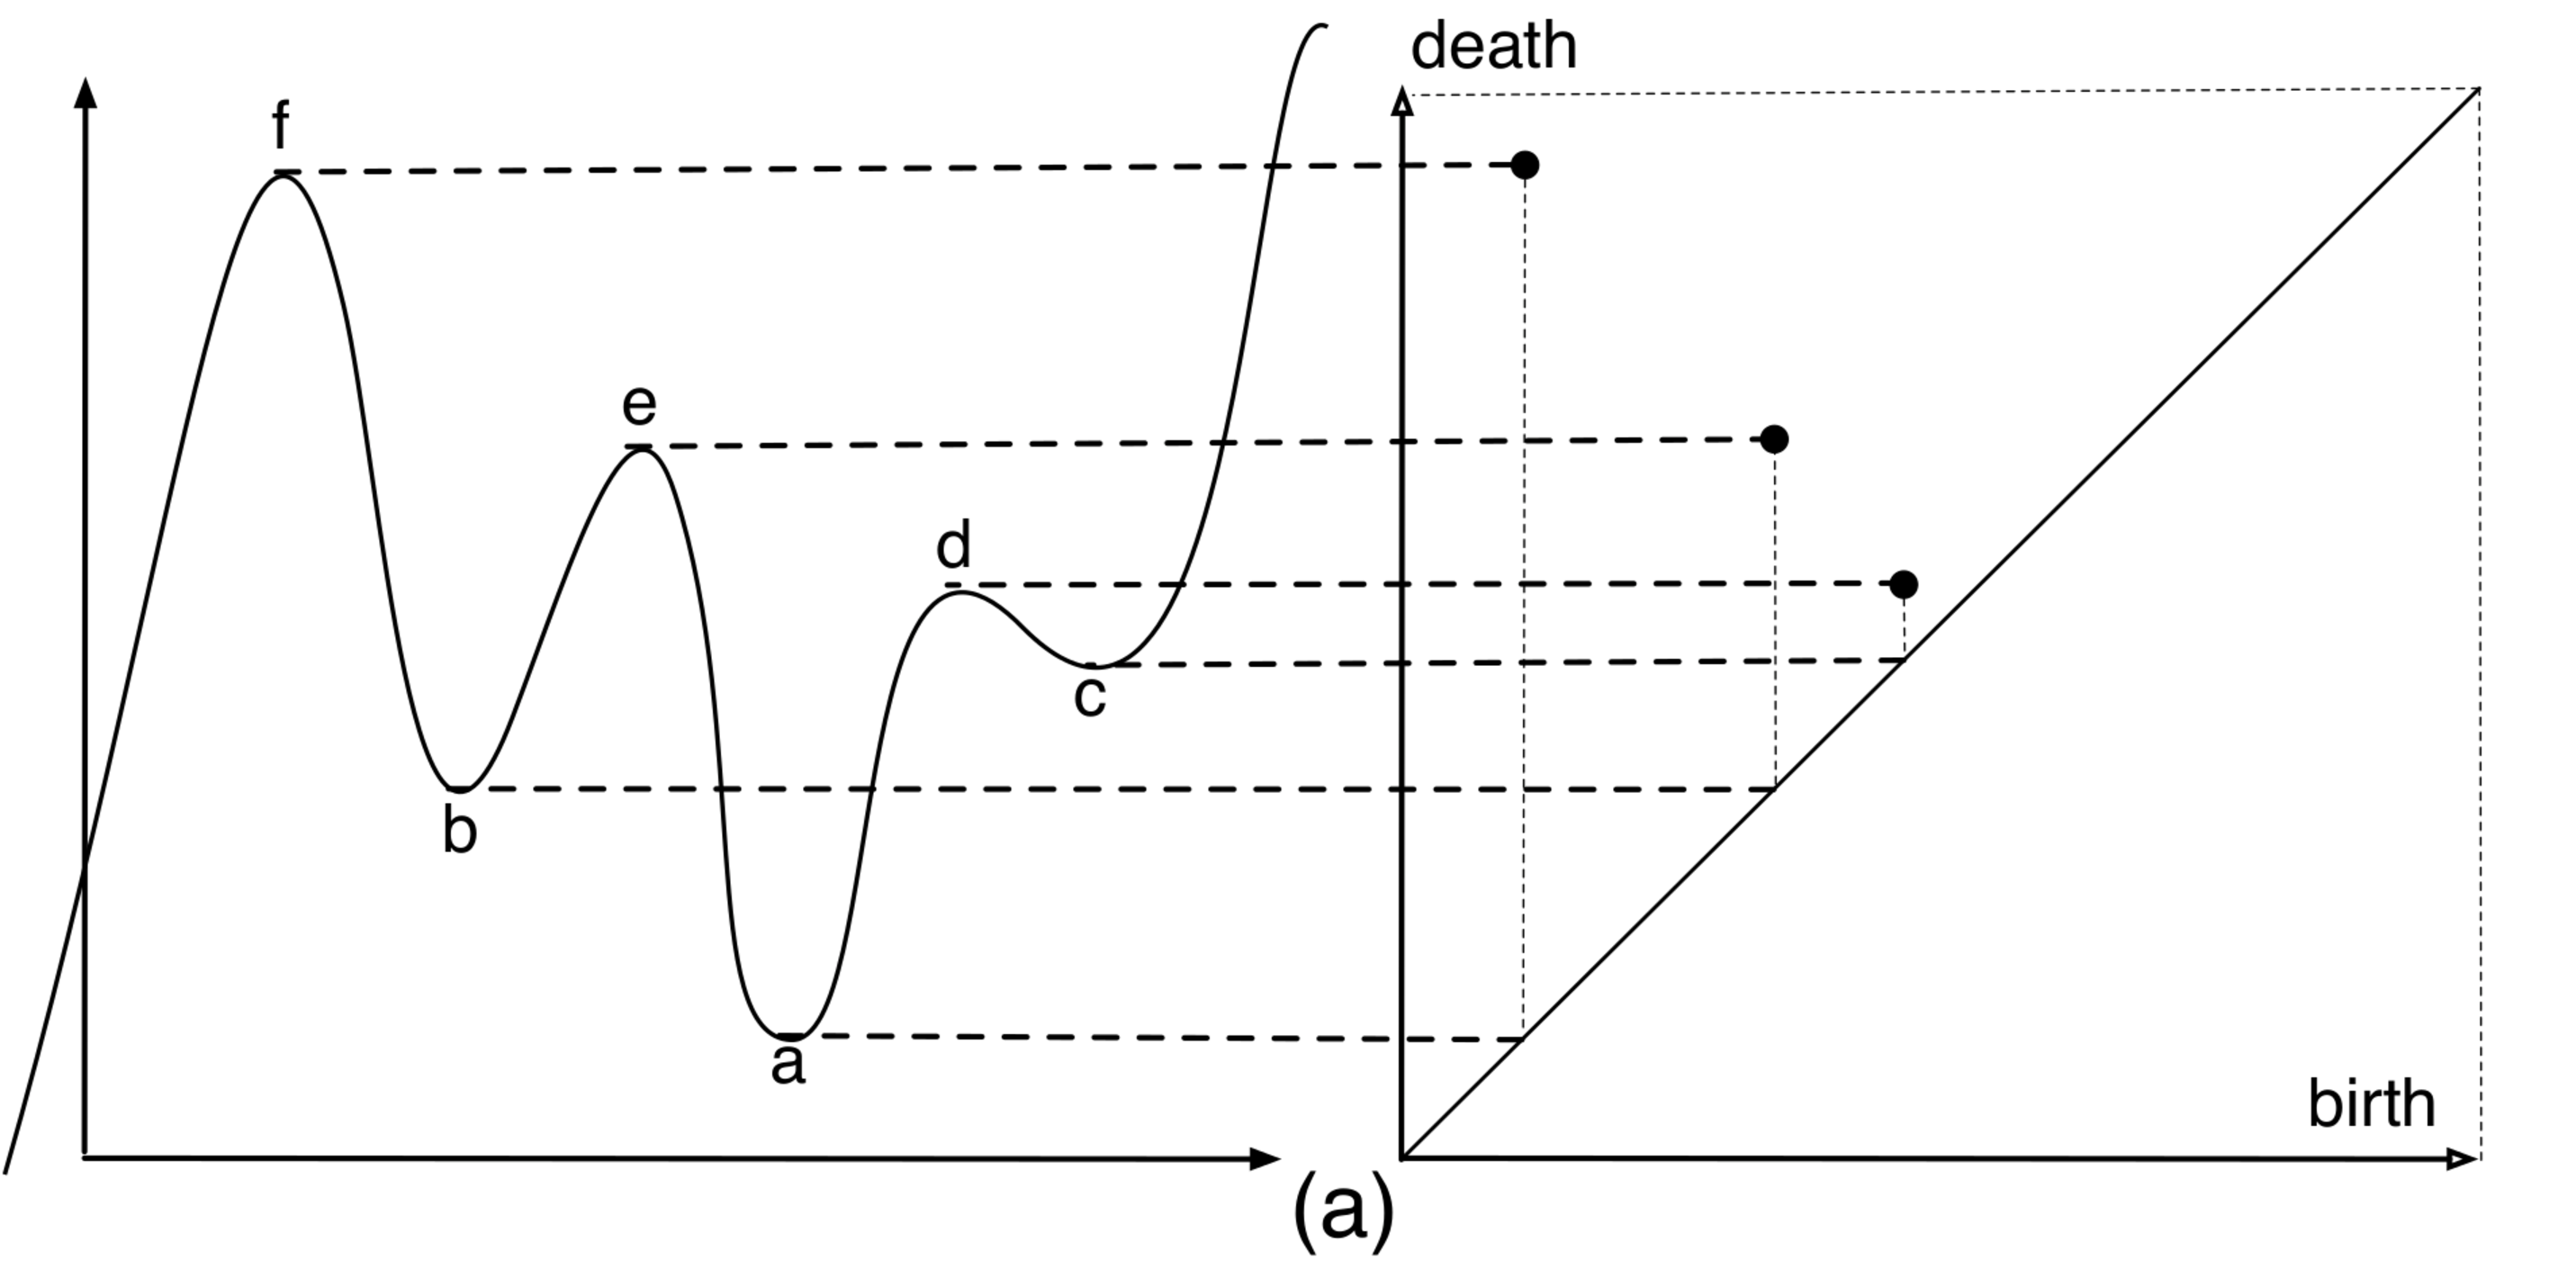
\includegraphics[width=0.65\textwidth]{figs/chap4/persistence-diagram}
  \caption[A one-dimensional function and its persistence diagram]{A one-dimensional Morse function with three local minima and three local maxima.
  %
  The critical points are paired, and each pair is encoded as a point in the persistence diagram on the right.}
  \label{fig:persistenceDiagram}
\end{figure}

As we increase in dimension, the pairing occurs only between critical points of consecutive indices.
%
That is, minima are paired with one-saddles, one-saddles are paired with two-saddles, and $(d-1)$-saddles are paired with local maxima.
%
Returning to our approximation, we have not yet described how to identify saddles.
%
As we are computing ascending and descending manifolds separately, we concern ourselves only with identifying one-saddles and $(d-1)$-saddles needed to cancel local minima and local maxima, respectively.
%
Saddle-saddle cancellations are omitted in this implementation.

We will describe briefly the process for finding $(d-1)$ saddles and performing merges for the descending manifolds case, and state that the ascending manifold case is performed the same way on $-f$.
%
We must first identify all points that lie on the boundary of two descending manifolds.
%
A point lies on the boundary of a descending manifold if its associated maximum is different from the associated maximum of one of its neighbors.
%
For each pair of adjacent descending manifolds, we identify the lowest valued point occurring on the shared boundary as the saddle point separating the two maxima.
%
With this information, the lower valued maximum is paired with the saddle and given a persistence equal to the function value difference between the two, and the higher valued maximum is named as the successor.
%
We then sort all potential cancellations by increasing persistence value and process them one at a time.
%
Each time we process a cancellation, we need to update the remaining potential cancellations in the list by replacing the merged maximum with its successor and update the persistence of the potential new cancellation accordingly.
%
If the successor is of larger value than the shared maximum on the new cancellation, we need to update only the partition label, but if the successor is of lower value, we must update the persistence of the new cancellation to be the function value of the saddle subtracted from the function value of the successor.
%
This process is performed recursively until a single partition exists for each connected component of the dataset.

% %
% In persistent homology, the connected components of complexes such as the \v{C}ech or Vietoris-Rips are tracked over an ever-increasing scale of values.
% %
% In order to understand this concept more thoroughly, we must describe how these complexes are constructed.
% %
% The \v{C}ech complex begins with a point set and a radius, $\epsilon$.
% %
% Each point is surrounded by a a ball of radius $\epsilon$.
% %
% A simplex is formed anytime there is an intersection of 2 or more balls.
% %
% Thus, we can track the birth and death of connected components in the complex as $\epsilon$ increases in size.
% %
% The Vietoris-Rips complex is similarly defined but relaxes the intersection property to include simplexes as long as there is a pairwise intersection among all of the balls.
% %
% In this way, we can attribute a persistence value to each connected component by subtracting the radius when the connected component is first discovered from the radius when the connected component disappears.

\section{Extremum Graphs}
\label{sec:extremumGraph}

The extremum graph was first introduced by Correa et al. as a simplified substructure of the Morse-Smale complex~\cite{CorreaLindstromBremer2011}.
%
Therefore, like the Morse-Smale complex, it can also be approximated for high-dimensional data~\cite{CorreaLindstromBremer2011,ThomasNatarajan2013}.
%
The approximation algorithm is a slightly modified version of the Morse complex algorithm presented in Section~\ref{sec:approximationMSC} used for computing the Morse-Smale complex.

We begin with a short recapitulation of the relevant Morse complex algorithm and then highlight the differences needed to compute the extremum graph.
%
Local maxima of the Morse complex are paired with $(d-1)$-index saddles occurring on the boundary of their respective descending manifolds in such a way that they can be canceled.
%
Such cancellations cause a merging of descending manifolds with the local maximum of the shared boundary, resulting in a simpler yet still valid Morse complex where gradient flow from the canceled maximum is redirected through the canceled saddle to the adjacent local maximum.
%
The order of these cancellations is typically chosen based on \textit{persistence}, that is the function value difference of the pair of canceled critical points.
%
The end result is a persistence hierarchy of Morse complexes of varying degrees of complexity.

The extremum graph is a variation of this persistence hierarchy that tracks not only the valid cancellations, but cancellations of potential \textit{strangulations}.
%
Strangulations occur when saddles are connected to the same extremum twice.
%
When processing the cancellations in order of increasing persistence, we may attempt to cancel a local maximum that has already been canceled.
%
Normally, these cancellations would be ignored, but for the extremum graph, we cancel only the saddle and assign its persistence value accordingly.
%
In the end, the hierarchy of the extremum graph is controlled by two parameters as opposed to the single persistence value used in the Morse/Morse-Smale complex setting.

A key observation made by Liu et al.~\cite{LiuWangMaljovec2019} is that the high-dimensional approximation algorithm for the extremum graph (and the Morse and Morse-Smale complex for that matter) does not require a precomputed graph model, which can be too large to fit in memory for large and high-dimensional datasets.
%
That is, edges can be streamed in and consumed as they are computed in two passes, one for the identification of local maximum labels and the second to identify $(d-1)$-saddles for persistence simplification.
%
This streaming process, coupled with the efficient computation of the empty region graphs presented in Chapter~\ref{ch:graphs}, has allowed us, for the first time, to perform topological analysis on datasets on the order of tens of millions of points in higher than three dimensions.

% \bibliography{\jobname}